\documentclass[11pt]{article}

\usepackage[a4paper, portrait, margin=0.9in]{geometry}
\setlength{\parskip}{1em}

\usepackage[hidelinks]{hyperref}

\usepackage{graphicx}
\graphicspath{ {./images/} }
\usepackage{caption}
\usepackage{subcaption}
\captionsetup[subfigure]{justification=centering}
\usepackage{wrapfig}

\title{COSC470 Research Project Report\\
\bigskip
Contour Splitting for Branching Structures in CT Image Reconstructions}
\author{Cameron Stevenson\\[0.5cm]{\small Supervisor: Ramakrishnan Mukundan}}

\begin{document}
\maketitle

\section{Overview}

overview text
Example citation \cite{mackay2019robust, mukundan2016reconstruction, pan2017comparison}.
Example URL \footnote{\url{https://github.com/cstevenson3/cosc470writing/blob/main/survey.pdf}}.

\section{Introduction}

introduction text

\section{Background}

background text

\subsection{Generic Methods}

generic methods text

\subsection{Correspondence Methods}

subsection preamble text

\subsubsection{Contour Correspondence}

contour correspondence text

Example list:
\begin{itemize}
\item item1
\item item2
\item item3
\end{itemize}

\subsubsection{Point Correspondence and Triangulation}

pc and t text

\begin{figure}[h]
     \centering
     \begin{subfigure}[b]{0.2\textwidth}
         \centering
         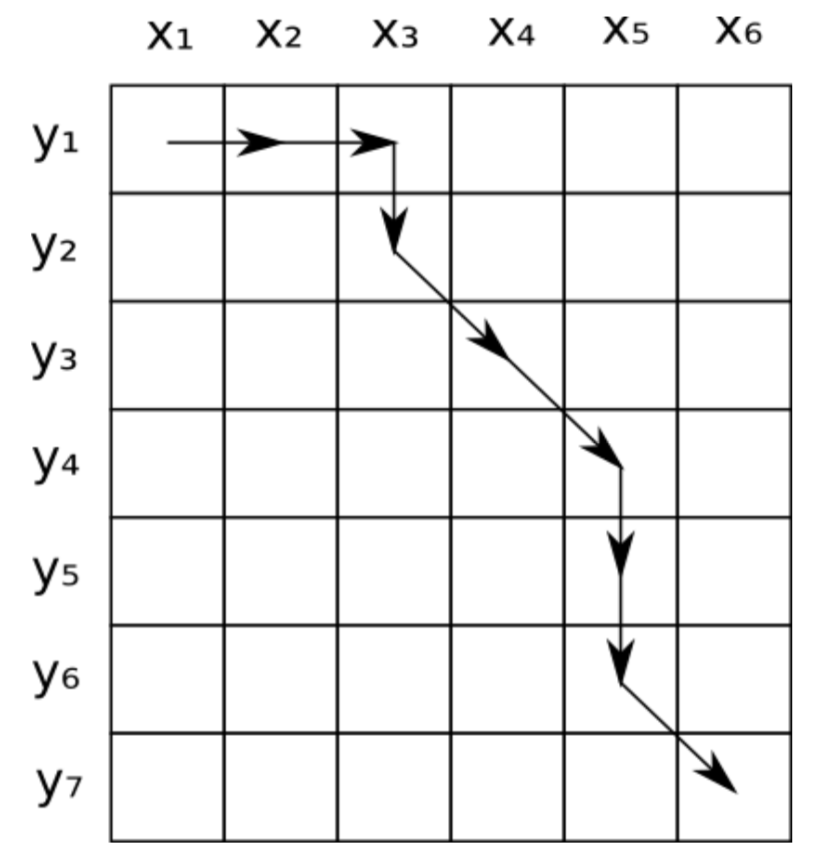
\includegraphics[width=\textwidth]{dtw1}
         \caption{DTW path through cost matrix}
         \label{fig:dtw1}
     \end{subfigure}
     \hfill
     \begin{subfigure}[b]{0.6\textwidth}
         \centering
         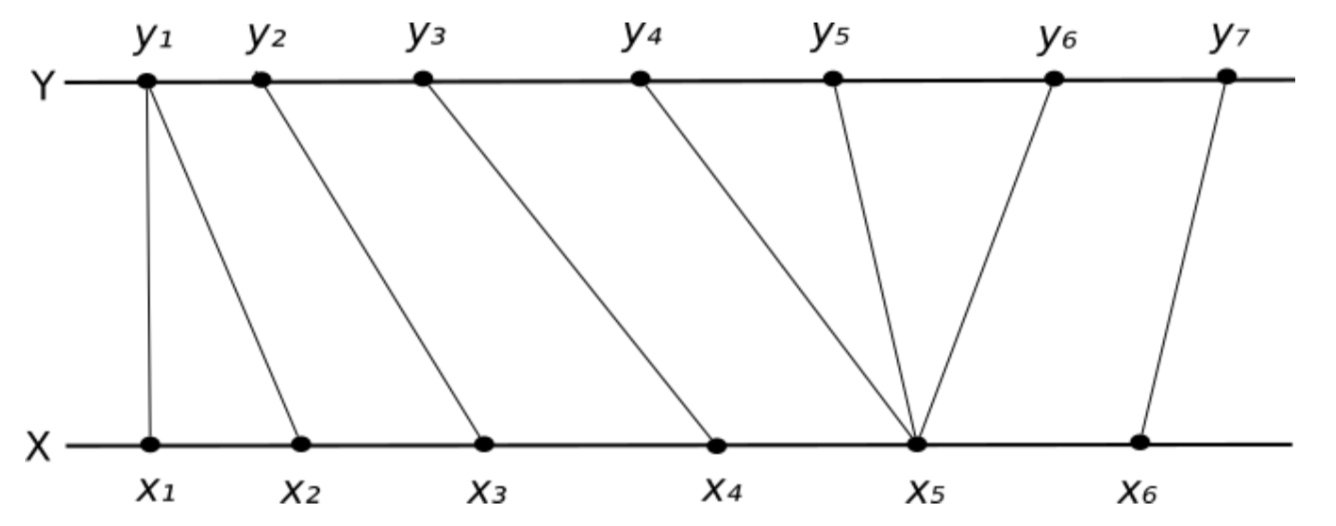
\includegraphics[width=\textwidth]{dtw2}
         \caption{DTW point correspondence}
         \label{fig:dtw2}
     \end{subfigure}
        \caption{Two examples of DTW paths on contours X and Y \cite{mackay2019robust}}
        \label{fig:dtw}
\end{figure}

text after figure declaration

\subsubsection{Branching Problem}

branching problem text

\section{Method}

method text

\subsection{Proposal}

\begin{wrapfigure}{r}{0.25\textwidth}
\centering
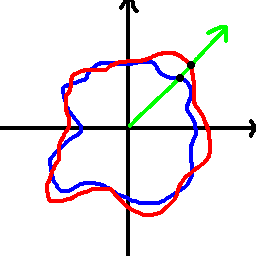
\includegraphics[width=0.2\textwidth]{pa}
\caption{Points matched by angle from shared centroid\label{fig:pa}}
\end{wrapfigure}

proposal text

Example figure ref (See Figure \ref{fig:pa}).

\subsection{Implementation}

pa text

\begin{figure}[h]
     \centering
     \begin{subfigure}[b]{0.22\textwidth}
         \centering
         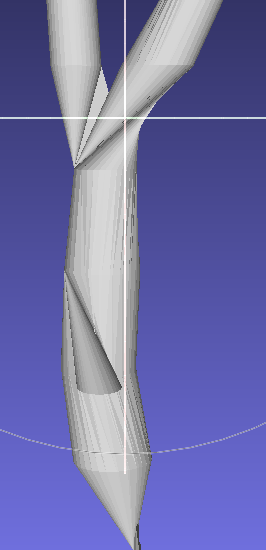
\includegraphics[width=\textwidth]{dtw10}
         \caption{DTW \linebreak}
         \label{fig:dtw10}
     \end{subfigure}
     \hfill
     \begin{subfigure}[b]{0.2\textwidth}
         \centering
         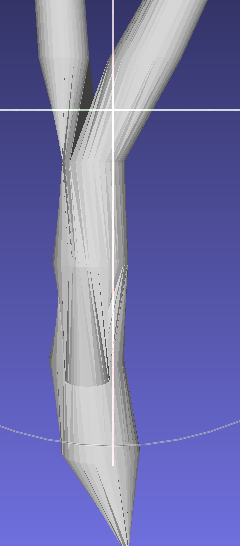
\includegraphics[width=\textwidth]{pa10ang00}
         \caption{Point angle, 0\% angle weight}
         \label{fig:pa10ang00}
     \end{subfigure}
     \hfill
     \begin{subfigure}[b]{0.195\textwidth}
         \centering
         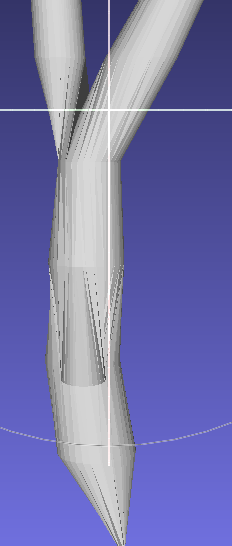
\includegraphics[width=\textwidth]{pa10ang50}
         \caption{Point angle, 50\% angle weight}
         \label{fig:pa10ang50}
     \end{subfigure}
     \hfill
     \begin{subfigure}[b]{0.2\textwidth}
         \centering
         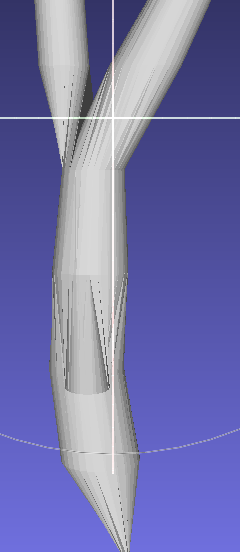
\includegraphics[width=\textwidth]{pa10ang100}
         \caption{Point angle, 100\% angle weight}
         \label{fig:pa10ang100}
     \end{subfigure}
        \caption{Reconstructions with 10 plane samples}
        \label{fig:plane10}
\end{figure}

\begin{figure}[h]
     \centering
     \begin{subfigure}[b]{0.215\textwidth}
         \centering
         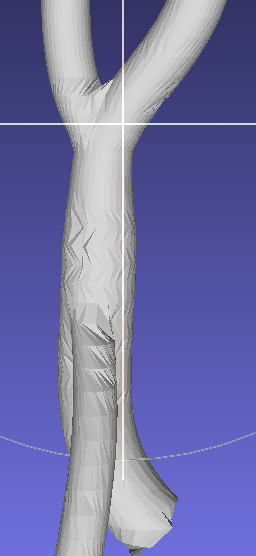
\includegraphics[width=\textwidth]{dtw50}
         \caption{DTW \linebreak}
         \label{fig:dtw50}
     \end{subfigure}
     \hfill
     \begin{subfigure}[b]{0.2\textwidth}
         \centering
         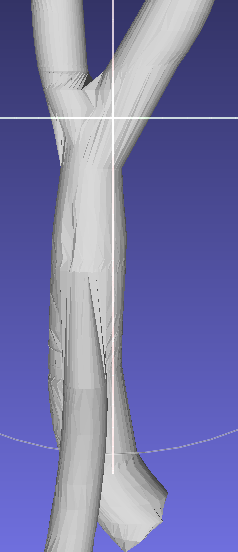
\includegraphics[width=\textwidth]{pa50ang00}
         \caption{Point angle, 0\% angle weight}
         \label{fig:pa50ang00}
     \end{subfigure}
     \hfill
     \begin{subfigure}[b]{0.205\textwidth}
         \centering
         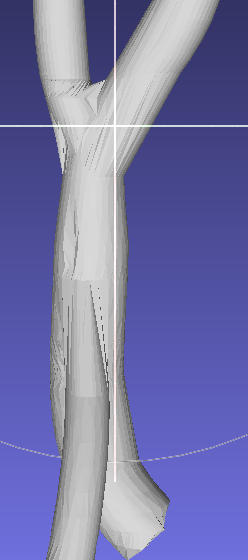
\includegraphics[width=\textwidth]{pa50ang50}
         \caption{Point angle, 50\% angle weight}
         \label{fig:pa50ang50}
     \end{subfigure}
     \hfill
     \begin{subfigure}[b]{0.2\textwidth}
         \centering
         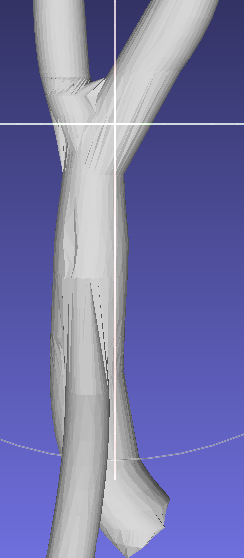
\includegraphics[width=\textwidth]{pa50ang90}
         \caption{Point angle, 90\% angle weight}
         \label{fig:pa50ang90}
     \end{subfigure}
        \caption{Reconstructions with 50 plane samples}
        \label{fig:plane50}
\end{figure}

\section{Analysis}

analysis text

\subsection{Ground Truth}

ground truth text

\subsection{Visual Results}

visual results text

\subsection{Measurements}

measurements text

\subsection{Summary}

summary text

\section{Conclusion}

conclusion text

\pagebreak
\bibliographystyle{IEEEtran}
\bibliography{references}

\section{Appendix}

\begin{figure}[h]
\centering
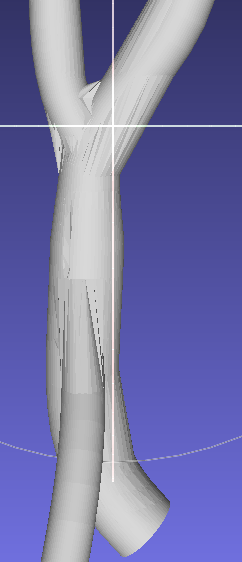
\includegraphics[width=0.29\textwidth]{mb}
\caption{Original multi branch model\label{fig:model}}
\end{figure}

\end{document}
